% Options for packages loaded elsewhere
\PassOptionsToPackage{unicode}{hyperref}
\PassOptionsToPackage{hyphens}{url}
%
\documentclass[
  english,
  man,floatsintext]{apa6}
\title{Analysing the effect of sibling number on input and output in the first 18 months: Supplementals}
\author{Catherine Laing\textsuperscript{1} \& Elika Bergelson\textsuperscript{2}}
\date{}

\usepackage{amsmath,amssymb}
\usepackage{lmodern}
\usepackage{iftex}
\ifPDFTeX
  \usepackage[T1]{fontenc}
  \usepackage[utf8]{inputenc}
  \usepackage{textcomp} % provide euro and other symbols
\else % if luatex or xetex
  \usepackage{unicode-math}
  \defaultfontfeatures{Scale=MatchLowercase}
  \defaultfontfeatures[\rmfamily]{Ligatures=TeX,Scale=1}
\fi
% Use upquote if available, for straight quotes in verbatim environments
\IfFileExists{upquote.sty}{\usepackage{upquote}}{}
\IfFileExists{microtype.sty}{% use microtype if available
  \usepackage[]{microtype}
  \UseMicrotypeSet[protrusion]{basicmath} % disable protrusion for tt fonts
}{}
\makeatletter
\@ifundefined{KOMAClassName}{% if non-KOMA class
  \IfFileExists{parskip.sty}{%
    \usepackage{parskip}
  }{% else
    \setlength{\parindent}{0pt}
    \setlength{\parskip}{6pt plus 2pt minus 1pt}}
}{% if KOMA class
  \KOMAoptions{parskip=half}}
\makeatother
\usepackage{xcolor}
\IfFileExists{xurl.sty}{\usepackage{xurl}}{} % add URL line breaks if available
\IfFileExists{bookmark.sty}{\usepackage{bookmark}}{\usepackage{hyperref}}
\hypersetup{
  pdftitle={Analysing the effect of sibling number on input and output in the first 18 months: Supplementals},
  pdfauthor={Catherine Laing1 \& Elika Bergelson2},
  pdflang={en-EN},
  pdfkeywords={Siblings, Lexical Development, Input Effects, Language Acquisition},
  hidelinks,
  pdfcreator={LaTeX via pandoc}}
\urlstyle{same} % disable monospaced font for URLs
\usepackage{graphicx}
\makeatletter
\def\maxwidth{\ifdim\Gin@nat@width>\linewidth\linewidth\else\Gin@nat@width\fi}
\def\maxheight{\ifdim\Gin@nat@height>\textheight\textheight\else\Gin@nat@height\fi}
\makeatother
% Scale images if necessary, so that they will not overflow the page
% margins by default, and it is still possible to overwrite the defaults
% using explicit options in \includegraphics[width, height, ...]{}
\setkeys{Gin}{width=\maxwidth,height=\maxheight,keepaspectratio}
% Set default figure placement to htbp
\makeatletter
\def\fps@figure{htbp}
\makeatother
\setlength{\emergencystretch}{3em} % prevent overfull lines
\providecommand{\tightlist}{%
  \setlength{\itemsep}{0pt}\setlength{\parskip}{0pt}}
\setcounter{secnumdepth}{-\maxdimen} % remove section numbering
% Make \paragraph and \subparagraph free-standing
\ifx\paragraph\undefined\else
  \let\oldparagraph\paragraph
  \renewcommand{\paragraph}[1]{\oldparagraph{#1}\mbox{}}
\fi
\ifx\subparagraph\undefined\else
  \let\oldsubparagraph\subparagraph
  \renewcommand{\subparagraph}[1]{\oldsubparagraph{#1}\mbox{}}
\fi
% Manuscript styling
\usepackage{upgreek}
\captionsetup{font=singlespacing,justification=justified}

% Table formatting
\usepackage{longtable}
\usepackage{lscape}
% \usepackage[counterclockwise]{rotating}   % Landscape page setup for large tables
\usepackage{multirow}		% Table styling
\usepackage{tabularx}		% Control Column width
\usepackage[flushleft]{threeparttable}	% Allows for three part tables with a specified notes section
\usepackage{threeparttablex}            % Lets threeparttable work with longtable

% Create new environments so endfloat can handle them
% \newenvironment{ltable}
%   {\begin{landscape}\centering\begin{threeparttable}}
%   {\end{threeparttable}\end{landscape}}
\newenvironment{lltable}{\begin{landscape}\centering\begin{ThreePartTable}}{\end{ThreePartTable}\end{landscape}}

% Enables adjusting longtable caption width to table width
% Solution found at http://golatex.de/longtable-mit-caption-so-breit-wie-die-tabelle-t15767.html
\makeatletter
\newcommand\LastLTentrywidth{1em}
\newlength\longtablewidth
\setlength{\longtablewidth}{1in}
\newcommand{\getlongtablewidth}{\begingroup \ifcsname LT@\roman{LT@tables}\endcsname \global\longtablewidth=0pt \renewcommand{\LT@entry}[2]{\global\advance\longtablewidth by ##2\relax\gdef\LastLTentrywidth{##2}}\@nameuse{LT@\roman{LT@tables}} \fi \endgroup}

% \setlength{\parindent}{0.5in}
% \setlength{\parskip}{0pt plus 0pt minus 0pt}

% Overwrite redefinition of paragraph and subparagraph by the default LaTeX template
% See https://github.com/crsh/papaja/issues/292
\makeatletter
\renewcommand{\paragraph}{\@startsection{paragraph}{4}{\parindent}%
  {0\baselineskip \@plus 0.2ex \@minus 0.2ex}%
  {-1em}%
  {\normalfont\normalsize\bfseries\itshape\typesectitle}}

\renewcommand{\subparagraph}[1]{\@startsection{subparagraph}{5}{1em}%
  {0\baselineskip \@plus 0.2ex \@minus 0.2ex}%
  {-\z@\relax}%
  {\normalfont\normalsize\itshape\hspace{\parindent}{#1}\textit{\addperi}}{\relax}}
\makeatother

% \usepackage{etoolbox}
\makeatletter
\patchcmd{\HyOrg@maketitle}
  {\section{\normalfont\normalsize\abstractname}}
  {\section*{\normalfont\normalsize\abstractname}}
  {}{\typeout{Failed to patch abstract.}}
\patchcmd{\HyOrg@maketitle}
  {\section{\protect\normalfont{\@title}}}
  {\section*{\protect\normalfont{\@title}}}
  {}{\typeout{Failed to patch title.}}
\makeatother

\usepackage{xpatch}
\makeatletter
\xapptocmd\appendix
  {\xapptocmd\section
    {\addcontentsline{toc}{section}{\appendixname\ifoneappendix\else~\theappendix\fi\\: #1}}
    {}{\InnerPatchFailed}%
  }
{}{\PatchFailed}
\keywords{Siblings, Lexical Development, Input Effects, Language Acquisition\newline\indent Word count: X}
\usepackage{lineno}

\linenumbers
\usepackage{csquotes}
\ifXeTeX
  % Load polyglossia as late as possible: uses bidi with RTL langages (e.g. Hebrew, Arabic)
  \usepackage{polyglossia}
  \setmainlanguage[]{english}
\else
  \usepackage[main=english]{babel}
% get rid of language-specific shorthands (see #6817):
\let\LanguageShortHands\languageshorthands
\def\languageshorthands#1{}
\fi
\ifLuaTeX
  \usepackage{selnolig}  % disable illegal ligatures
\fi


\shorttitle{Effect of sibling number on language: Supplementals}

\authornote{

Correspondence concerning this article should be addressed to Catherine Laing, Department of Language and Linguistic Science, University of York, Heslington, York, UK, YO10 5DD. E-mail: \href{mailto:catherine.laing@york.ac.uk}{\nolinkurl{catherine.laing@york.ac.uk}}

}

\affiliation{\vspace{0.5cm}\textsuperscript{1} University of York, York, UK\\\textsuperscript{2} Duke University, Durham, NC, USA}

\begin{document}
\maketitle

\hypertarget{s1-effect-of-siblings-on-infants-input---audio-recordings}{%
\subsection{S1: Effect of siblings on infants' input - audio recordings}\label{s1-effect-of-siblings-on-infants-input---audio-recordings}}

Our main results analyse input data from the hour-long video recordings taken in the home on a monthly basis. We re-ran our analysis using the home-recorded audio data, which captures a snapshot from a daylong recording using a LENA device (\url{https://www.lena.org/}) worn in a vest. In this case, age but not sex was included in both models.

Outputs from model comparisons and full model outputs including estimates are shown in Tables \ref{tab:table-model-comparisons-audio} and \ref{tab:table-input-model-summary-audio}. Results were consistent with the video data for object presence, but not overall input.

\begin{longtable}[t]{cccc}
\caption{\label{tab:table-model-comparisons-audio}Full model output from linear mixed effects regression models comparing our two input measures in relation to sibling group in the audio data. Age in months was included as a fixed effect; subject was included as a random effect.}\\
\toprule
Model & Df & Chisq & p value\\
\midrule
Caregiver input & 2 & 3.00 & 0.22\\
Object presence & 2 & 23.83 & 0.00\\
\bottomrule
\end{longtable}

\begin{longtable}[t]{ccccccc}
\caption{\label{tab:table-input-model-summary-audio}Full model output from linear mixed effects regression models comparing our two input measures (object words produced in caregiver input and object presence) over time in relation to sibling group, for the audio data. Age in months was included as a fixed effect in both models and subject was included as a random effect.}\\
\toprule
Variable & Effect & Estimate & Std. Error & df & t value & p value\\
\midrule
Caregiver input & Intercept & 6.15 & 0.13 & 83.68 & 46.58 & <0.001\\
 & SibGroupOne & 0.13 & 0.18 & 42.99 & 0.73 & 0.469\\
 & SibGroup2+ & -0.26 & 0.20 & 42.99 & -1.26 & 0.213\\
 & month & -0.04 & 0.01 & 472.00 & -6.01 & <0.001\\
\midrule
Object presence & Intercept & 0.42 & 0.03 & 222.79 & 16.82 & <0.001\\
\addlinespace
 & SibGroupOne & -0.08 & 0.03 & 43.02 & -3.20 & 0.003\\
 & SibGroup2+ & -0.16 & 0.03 & 43.01 & -5.46 & <0.001\\
 & month & 0.02 & 0.00 & 472.05 & 9.59 & <0.001\\
\bottomrule
\end{longtable}

\newpage

\hypertarget{s2-speakers-in-the-dataset}{%
\subsection{S2: Speakers in the dataset}\label{s2-speakers-in-the-dataset}}

The table below provides a summary of which two caregivers produced the most words in each video recording analyized in the main manuscript. This was usually the mother and/or the father.

\begin{longtable}[t]{ccc}
\caption{\label{tab:table-speakers-sessions}Numer of sessions in which each adult speaker is one of the two main caregivers. There were 344 hour-long video recordings in total across the 43 infants in the dataset. In the case where the infant had two mothers, their data was aggregated into the 'Mother' category; in all but two sessions from this family, the two mothers were the two main caregivers.}\\
\toprule
Speaker & Caregiver 1 & Caregiver 2\\
\midrule
Mother & 425 & 26\\
Father & 62 & 121\\
Grandmother & 21 & 32\\
Babysitter & 5 & 4\\
Grandfather & 1 & 9\\
\addlinespace
Other Adult & 1 & 11\\
Aunt & 0 & 8\\
Uncle & 0 & 3\\
\bottomrule
\end{longtable}

\newpage

\hypertarget{s3-correlations-with-maternal-factors}{%
\subsection{S3: Correlations with maternal factors}\label{s3-correlations-with-maternal-factors}}

There were no correlations between sibling number or child word production and maternal age/education. See Figure \ref{fig:Figure-correlations}.

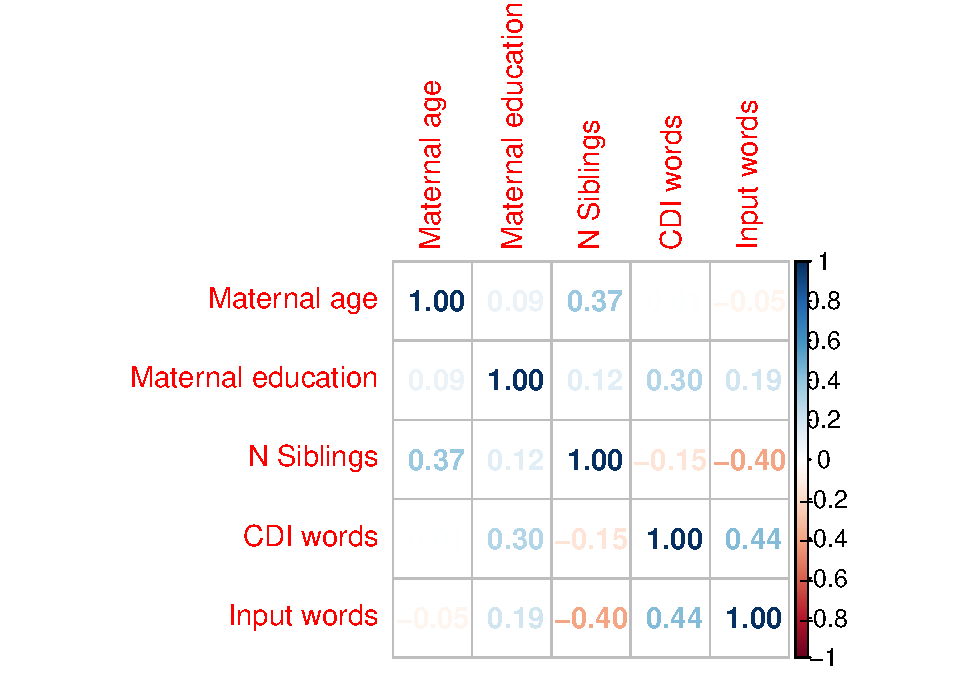
\includegraphics{SiblingsStudy_SupplementaryData_files/figure-latex/Figure-correlations-1.pdf}
\newpage

\hypertarget{s4-discrete-sibling-number}{%
\subsection{S4: Discrete sibling number}\label{s4-discrete-sibling-number}}

As discrete sibling number, as well as sibling group, revealed siblings to be a significant predictor of vocabulary size at 18 months, we re-ran our input models using discrete sibling number as a fixed effect, instead of sibling group. Outputs from model comparisons and full model outputs including estimates are shown in Tables \ref{tab:table-model-comparisons-discrete} and \ref{tab:table-input-model-summary-discrete}. Results were consistent with those reported for sibling group suggesting both characterizations of siblinghood capture similar relationships among our variables.

\begin{longtable}[t]{cccc}
\caption{\label{tab:table-model-comparisons-discrete}Full model output from linear mixed effects regression models comparing our two input measures in relation to discrete sibling number. Age in months was included as a fixed effect; subject was included as a random effect.}\\
\toprule
Model & Df & Chisq & p value\\
\midrule
Caregiver input & 1 & 7.02 & 0.01\\
Object presence & 1 & 22.98 & 0.00\\
\bottomrule
\end{longtable}

\begin{longtable}[t]{ccccccc}
\caption{\label{tab:table-input-model-summary-discrete}Full model output from linear mixed effects regression models comparing our two input measures (object words produced in caregiver input and object presence) over time in relation to discrete sibling number. Age in months was included as a fixed effect in both models and subject was included as a random effect.}\\
\toprule
Variable & Effect & Estimate & Std. Error & df & t value & p value\\
\midrule
Caregiver input & Intercept & 4.83 & 0.13 & 79.35 & 38.53 & <0.001\\
 & Siblings6 & -0.16 & 0.06 & 42.99 & -2.76 & 0.008\\
 & month & 0.04 & 0.01 & 472.04 & 6.38 & <0.001\\
 & sexM & -0.20 & 0.13 & 43.00 & -1.51 & 0.138\\
\midrule
Object presence & Intercept & 0.59 & 0.03 & 218.11 & 22.45 & <0.001\\
\addlinespace
 & Siblings6 & -0.07 & 0.01 & 43.00 & -5.51 & <0.001\\
 & month & 0.01 & 0.00 & 472.13 & 2.87 & 0.004\\
\bottomrule
\end{longtable}

\newpage

\hypertarget{s5-possible-outlier-for-input-data-removed}{%
\subsection{S5: Possible outlier for input data removed}\label{s5-possible-outlier-for-input-data-removed}}

One infant heard substantially more nouns in their input and nouns with object presence than the other 42 infants in the main sample for four of their recording sessions. We retain this infant in the main analysis, but confirm here that results were consistent when this child was removed from the analysis of input data (n=42). Results were consistent with those reported for sibling group. See Tables \ref{tab:table-model-comparisons-red} and \ref{tab:table-input-model-summary-red}.

\begin{longtable}[t]{cccc}
\caption{\label{tab:table-model-comparisons-red}Full model output from linear mixed effects regression models comparing our two input measures in relation to sibling group, with one infant removed who was identified as hearing substantially more input speech (3SDs above the group mean) in 4 recordings (n=42). Age in months was included as a fixed effect; subject was included as a random effect.}\\
\toprule
Model & Df & Chisq & p value\\
\midrule
Caregiver input & 2 & 10.26 & 0.01\\
Object presence & 2 & 29.34 & 0.00\\
\bottomrule
\end{longtable}

\begin{longtable}[t]{ccccccc}
\caption{\label{tab:table-input-model-summary-red}Full model output from linear mixed effects regression models comparing our two input measures (object words produced in caregiver input and object presence) over time in relation to sibling group, with one infant removed who was identified as hearing substantially more input speech (3SDs above the group mean) in 4 recordings (n=42). Age in months was included as a fixed effect in both models and subject was included as a random effect.}\\
\toprule
Variable & Effect & Estimate & Std. Error & df & t value & p value\\
\midrule
Caregiver input & Intercept & 4.76 & 0.12 & 80.32 & 38.13 & <0.001\\
 & SibGroupOne & 0.06 & 0.13 & 42.03 & 0.42 & 0.679\\
 & SibGroup2+ & -0.46 & 0.15 & 41.99 & -3.03 & 0.004\\
 & month & 0.04 & 0.01 & 461.06 & 6.24 & <0.001\\
 & sexM & -0.24 & 0.12 & 42.01 & -2.02 & 0.049\\
\midrule
\addlinespace
Object presence & Intercept & 0.61 & 0.03 & 202.66 & 22.20 & <0.001\\
 & SibGroupOne & -0.11 & 0.03 & 42.09 & -3.82 & <0.001\\
 & SibGroup2+ & -0.20 & 0.03 & 42.00 & -6.28 & <0.001\\
 & month & 0.01 & 0.00 & 461.15 & 2.91 & 0.004\\
\bottomrule
\end{longtable}


\end{document}
